% tipo de documento
\documentclass{article}

% idioma de los macros
\usepackage[spanish]{babel}

% formato de página
\usepackage[letterpaper, margin = 1.5cm]{geometry}

% manejo de ecuaciones
\usepackage{amsmath}

% imágenes
\usepackage{graphicx}
\graphicspath{{./img/}}

% encabezado
\title{
    Autómatas y Lenguajes Formales \\
    Tarea Examen Parcial 4
}

\date{
    Fecha de entrega: 5 de junio
}

\author{blank}

% documento
\begin{document}
    \maketitle

    \begin{enumerate}
        \item (2 pts) La siguiente máquina de Turing $M_f$ calcula una función
        $f$ que recibe cadenas de $\{a, b\}^{\star}$ y devuelve cadenas de 
        $\{a, b\}^{\star}$.
        \begin{center}
            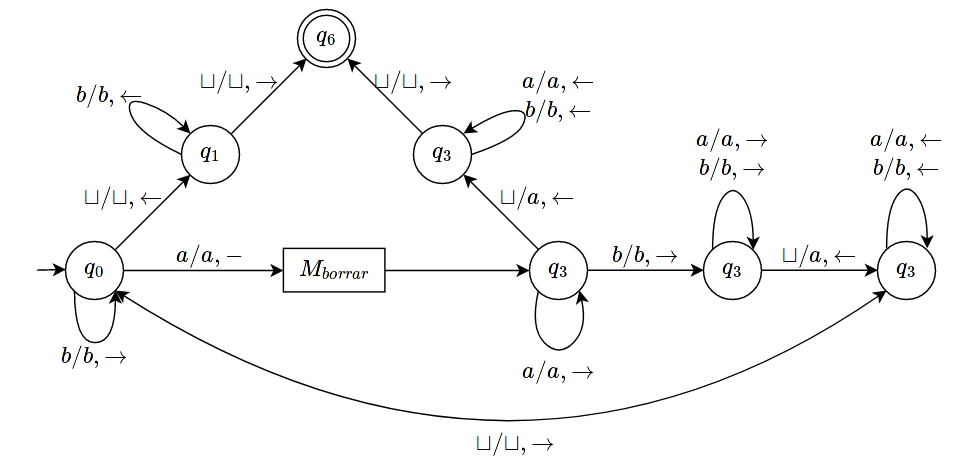
\includegraphics[scale=0.5]{automata1.png}
        \end{center}
        \begin{enumerate}
            \item Define al macro $M_{borrar}$ dando la table de transiciones,
            el diagrama y explicando el diseño.
            \item Describe $f(w), x \in \{a, b\}^{\star}$. ¿En qué posición 
            acaba la cabeza?
        \end{enumerate}

        \item (1 pt) Dada la siguiente codificación de una máquina de Turing sobre el 
        alfabeto $\Sigma = \{0, 1\}$
        \begin{align*}
            &010110101101001011101011101001010111010110 \\
            &01110110111101101001111010111111011011001110111011111011010 \\
            &01111101011111101110110011111101101111110110110 \\
            &0111111011101111110111011001111110101101010 \\
        \end{align*}
        \begin{enumerate}
            \item Decodifica la máquina
            \item ¿Qué hace la máquina?
            \item ¿En dónde termina la cabeza?
        \end{enumerate}
        \item (1.5 pts) ¿Cómo se simula un autómata de pila usando una máquina 
        de Turing?\\
        Explica la idea ejemplificando la creación de una máquina de Turing que
        simula a un autómata de pila que acepte al lenguaje 
        $L = \{a^ib^jc^k | i, j, k \geq 0, i + j = k\}$ 
        
        \item (i.5 pts) Decide si $w_1 = aba$ y $w_2 = bbb$ pertenece a $L(G)$.
        \begin{align*}
            &S \rightarrow \ X | Y \\
            &X \rightarrow \ aZb | bZa \\
            &Z \rightarrow \ aZb | bZa | \varepsilon \\
            &Y \rightarrow \ aB | bA \\
            &A \rightarrow \ a | aA \\
            &B \rightarrow \ b
        \end{align*}
        Para hacer esto, primero para $G$ a $FNC$ mostrando cada paso.

        \item (2 pts) Considere las siguiente producciones de comandos.
        \begin{align*}
            &\texttt{Cmd ::= print ( Exp ) | Cmd ; Cmd | if Exp then Cmd else Cmd} \\
            &\texttt{Exp ::= Num | Exp + Exp} \\
            &\texttt{Num ::= Dig | Num Dig} \\
            &\texttt{Dig ::= 0 | 1 | ... | 9}
        \end{align*}

        \begin{enumerate}
            \item Muestre que la gramática es ambigua.
            \item Existen al menos dos tipos de ambiguedad. Ejemplifique cada uno.
            \item De las ambiguedades, ¿cuáles son relevantes semánticamente? 
            Supongo que el operador $;$ es asociativo.
        \end{enumerate}
        
        \item[\textbf{Extra}] (2 pts) Considere la siguiente gramática.
        \[\texttt{Type ::= int | bool | \^\ Type | Type * Type | ( Type )}\]
        donde \texttt{int, bool, \^\ , (} y \texttt{)} son símbolos terminales.

        \begin{enumerate}
            \item Muestre que la gramática es ambigua.
            \item Defina una grmática no ambigua que genere el mismo lenguaje.
            \item Describa las reglas de precedencia y asociatividad para su
            lenguaje.
        \end{enumerate}
    \end{enumerate}
\end{document}